\chapter{Kiến Thức Nền Tảng}
\ifpdf
    \graphicspath{{Chapter2/Chapter2Figs/PNG/}{Chapter2/Chapter2Figs/PDF/}{Chapter2/Chapter2Figs/}}
\else
    \graphicspath{{Chapter2/Chapter2Figs/EPS/}{Chapter2/Chapter2Figs/}}
\fi

\begin{quote}

%Trong chương này, chúng tôi sẽ trình bày những kiến thức nền tảng trên ba chủ đề chính bao gồm\textit{Mạng nơ-ron hồi quy (Recurrent neural network)} và biến thể của nó \textit{Long short-term memory} với khả năng giải quyết vấn đề về các \textit{phụ thuộc dài hạn} (Long term dependencies). Chúng tôi cũng trình bày về mô hình dịch máy nơ-ron dựa trên kiến trúc bộ mã hóa - bộ giải mã đã được đề cập đến trong chương giới thiệu. Những kiến thức được trình bày trong chương này cung cấp những nền tảng cũng như phân tích các vấn đề mà kiến trúc bộ mã hóa - bộ giải mã gặp phải để đi đến chương tiếp theo về cơ chế \textit{Attention} trong dịch máy nơ-ron.

Trong chương này, chúng tôi sẽ trình bày những kiến thức nền tảng trên ba chủ đề bao gồm mạng nơ-ron hồi quy, mô hình ngôn ngữ nơ-ron và mô hình dịch máy nơ-ron. Mạng nơ-ron hồi quy (RNN) là xương sống của dịch máy nơ-ron. Nó được sử dụng để làm cả bộ mã hóa lẫn bộ giải mã. Ứng với mỗi vai trò, RNN sẽ có một thiết kế riêng. Một phiên bản cải tiến của RNN là \textit{Long short-term memory} cũng được chúng tôi trình bày, phiên bản này giúp cho việc huấn luyện RNN trở nên dễ dàng hơn. Sau đó, dựa trên những kiến thức về mạng nơ-ron hồi quy, chúng tôi nói về khái niệm \textit{mô hình ngôn ngữ hồi quy} với khả năng \textit{tạo ra ngôn ngữ}, là bước quan trọng trong dịch máy nơ-ron. Cuối cùng, chúng tôi cũng trình bày về mô hình dịch máy nơ-ron theo kiến trúc bộ mã hóa - bộ giải mã với RNN và mô hình ngôn ngữ hồi quy là những thành phần nền tảng.

\end{quote}
\section{Mạng nơ-ron hồi quy (Recurrent neural network)}

Trong bài toán dịch máy với dữ liệu văn bản, ta biết rằng những từ trong một câu hoặc một đoạn văn không bao giờ là độc lập với nhau. Ví dụ như trong câu sau \textit{Paris là thủ đô của nước \_\_}. Dễ biết được rằng từ trong chỗ trống sẽ là \textit{Pháp}. Tuy nhiên, trong trường hợp không đọc những từ phía trước, chúng ta không thể nào đoán được từ trong chỗ trống là gì. Điều này có nghĩa là một từ luôn có mối liên hệ với những từ phía trước nó và chúng có một thứ tự. Ta gọi loại dữ liệu có thứ tự là dữ liệu chuỗi.

\textit{Mạng nơ-ron hồi quy (recurrent neural network)} \cite{elman1990} gọi tắt là \textit{RNN} là một nhánh của Mạng nơ-ron nhân tạo được thiết kế đặc biệt cho việc mô hình hóa loại dữ liệu chuỗi. Lý do RNN thích hợp là vì nó tận dụng được tính chất tuần tự của loại dữ liệu này. Xét một chuỗi $x={x_1,x_2,...,x_n}$ và đầu ra tương ứng của nó $y={y_1,y_2,...,y_n}$, ta muốn học một ánh xạ $f: x \mapsto y$. Trong trường hợp này, một mạng nơ-ron truyền thẳng chỉ có thể ánh xạ một đầu vào $x_i$ sang một đầu ra $y_i$. Trong khi đó, trên lý thuyết, một RNN hoàn toàn có thể tận dụng toàn bộ lịch sử của những đầu vào trước đó $x_{1 \mapsto i}$ vào việc tính toán $y_i$. Để làm được việc này, RNN với các kết nối vòng cho phép nó sở hữu một loại "bộ nhớ". Bộ nhớ này sẽ tồn tại trong RNN và tác động đến đầu ra của nó. %Hình \ref{fig_rnn_loop} thể hiện kết nối vòng của RNN.

%\begin{figure}
%	\centering
%	\includegraphics[width=0.3\textwidth]{rnn_loop}
%	\caption[Mô hình RNN đơn giản]{Mô hình RNN đơn giản với kết nối vòng, \textbf{$h$} được xem như bộ nhớ được luân chuyển trong RNN}
%	\label{fig_rnn_loop}
%\end{figure}

Với mỗi đầu vào $x_i$ trong chuỗi $x={x_1,x_2,...,x_n}$, RNN cập nhật bộ nhớ để tạo ra một trạng thái ẩn $h_i$. Vector này có thể được xem như là một đại diện cho tập các đầu vào tại thời điểm trước đó $x_{1 \mapsto i}$. Điểm mấu chốt để RNN hoạt động là cách nó cập nhật trạng thái ẩn. Ở dạng đơn giản nhất, RNN định nghĩa công thức cập nhật trạng thái ẩn của nó như sau:
\begin{equation} \label{basicRnnEquation}
	h_t = f \left(h_{t-1}, x_t \right)
\end{equation}

Trong công thức trên, hàm $f$ tính trạng thái ẩn ở thời điểm $t$ dựa trên trạng thái ẩn trước đó $h_{t-1}$ và đầu vào $x_t$. Thông thường, hàm $f$ là một hàm phi tuyến như hàm \textit{sigmoid} hay hàm \textit{tanh}. Xét một RNN với công thức cụ thể như sau:  
\begin{equation} \label{rnnWithTanh}
	h_t = tanh \left(W_{xh} x_t + W_{hh}h_{t-1} + b_h \right)
\end{equation}

Ở đây $W_{xh}$, $W_{hh}$ và $b_h$ là các tham số học của mô hình. Ta thấy hàm định nghĩa $h_t$ là một mạng nơ-ron truyền thẳng với $W_{xh}$ là ma trận trọng số kết nối kết nối đầu vào và trạng thái ẩn. $W_{hh}$ là ma trận kết nối trạng thái ẩn và chính nó, $b_h$ là vector bias của trạng thái ẩn. Tại thời điểm bắt đầu, trạng thái ẩn $h_0$ có thể được khởi tạo bằng 0 hoặc là một vector chứa tri thức có sẵn như trường hợp của bộ giải mã như chúng tôi đã đề cập trong chương 1.

Tại mỗi thời điểm $t$, tùy vào mục tiêu cụ thể của quá trình học mà RNN có thể có thêm một đầu ra $y_t$. Trong ngữ cảnh bài toán dịch máy nơ-ron, đầu ra của RNN trong quá trình giải mã chính là một từ trong ngôn ngữ đích. Với mục tiêu đó, đầu ra dự đoán của RNN $\hat{y}_t$ sẽ có dạng là một phần phối xác suất trên tập từ vựng ở ngôn ngữ đích. Phân phối này nhằm dự đoán sự xuất hiện của từ $\hat{y}_t$ trong tập từ vựng.
\begin{equation} \label{rnnOuputSoftmax}
	s_t = W_{hy}h_t + b_y
\end{equation}
\begin{equation} \label{rnnOuputSoftmaxDistribution}
	\hat{y_t} = softmax(s_t)
\end{equation}

Trong công thức trên, $W_{hy}$, $b_y$ là những tham số khác của mô hình. $W_{hy}$ là ma trận trọng số kết nối đầu ra, $b_y$ là vector bias ở đầu ra. $s_t$ là một vector có độ dài bằng với là số lượng từ vựng trong ngôn ngữ đích. Vector này được chuẩn hóa thành một phân phối xác suất $\hat{y_t}$ bằng một hàm \textit{softmax}.

Để ý rằng các ma trận trọng số $W_{xh}$, $W_{hh}$, $W_{hy}$ và các vector bias $b_h$, $b_y$ là duy nhất cho toàn bộ mô hình. Có nghĩa là khi những tham số này được học, bất kỳ một đầu vào nào cũng đều sử dụng chung một bộ tham số. Điều này chính là \textit{sự chia sẻ tham số (parameters sharing)} trong mạng nơ-ron hồi quy. Chia sẻ tham số khiến cho mô hình học dễ dàng hơn, nó giúp cho RNN có thể xử lý chuỗi đầu vào với độ dài bất kỳ mà không làm tăng độ phức tạp của mô hình. Quan trọng hơn, nó giúp ích cho việc tổng quát hóa. Đây chính là điểm đặc biệt của RNN so với mạng nơ-ron truyền thẳng.

\subsection{Huấn luyện mạng nơ-ron hồi quy}



\subsection{Long short-term memory}

Hochreiter và Schmidhuber [1997] đã giới thiệu mô hình LSTM chủ yếu ở để khắc phục vấn đề biến mất gradient. Mô hình này tương tự với mô hình 

%Ta hãy xem xét một ví dụ về não người trong quá trình tạo ra các hành động. Khi chạm tay vào vật nóng, não sẽ tạo ra một tín hiệu để ra lệnh cho cơ thể chúng ta rút tay lại. Không những thế, cảm giác nóng sẽ chuyển hóa thành một suy nghĩ. Suy nghĩ này lại được truyền qua não và dựa trên thông tin của giác quan, ta tiếp tục thực hiện một hành động khác. Ví dụ nhúng tay vào nước khi biết có nước gần đó. Có thể hình dung một cách đơn giản rằng não người hoạt động như một hàm \textit{hồi quy}, nó nhận vào thông tin của giác quan và một suy nghĩ nội tại để tạo ra một hành động và suy nghĩ mới. Suy nghĩ mới này bao gồm cả những suy nghĩ trước đó. Cách hoạt động của não người trong ví dụ trên cũng chính là cách mà RNN làm việc. Trong đó, tại mỗi thời điểm, thông tin về giác quan được xem như đầu vào của RNN và đầu ra là một hành động. "Suy nghĩ" hoạt động như một loại bộ nhớ giúp RNN lưu giữ thông tin về bối cảnh, là những gì mà nó đã xử lý trong quá khứ. Việc sở hữu một loại "bộ nhớ" khiến RNN trở thành mô hình phù hợp cho dữ liệu chuỗi.
%Trong thực tế, mạng nơ-ron hồi quy được áp dụng thành công trong các bài toán mô hình hóa ngôn ngữ \cite{mikolovLM}.

%\begin{figure}
%	\centering
%	\includegraphics[width=0.3\textwidth]{rnn_loop}
%	\caption[Mô hình RNN đơn giản]{Mô hình RNN đơn giản}
%	\label{fig_rnn_loop}
%\end{figure}

%Hình \ref{fig_rnn_loop} mô tả cấu trúc cơ bản của RNN. Trong đó $x_t$ và $y_t$ lần lượt là đầu vào và đầu ra của RNN tại thời điểm (time step) $t$. $A$ được gọi là một \textit{tế bào RNN (RNN cell)} , thường là một mạng nơ-ron truyền thẳng. Tại mỗi thời điểm $t$, tế bào RNN sẽ tính toán dựa trên đầu vào $x_t$ và một vector $h$ được gọi là \textit{trạng thái ẩn (hidden state)}, là kết quả của quá trình tính toán tại thời điểm ngay trước đó. Sau khi tính toán, tế bào này tạo ra một trạng thái ẩn mới và trạng thái ẩn này tiếp tục được đưa vào mạng cho những tính toán ở thời điểm sau đó. Quá trình này được thể bằng một vòng lặp trong bản thân tế bào RNN. Lưu ý rằng đường nét đứt bao quanh $x_t$, $y_t$ cho biết đầu vào và đầu ra của tế bào RNN là không bắt buộc.

%\begin{figure}
%	\centering
%	\includegraphics[width=\textwidth]{rnn_unfolded}
%	\caption[Mô hình RNN được giàn trải]{Mô hình RNN được giàn trải}
%	\label{fig_rnn_unfolded}
%\end{figure}

%TODO explain RNN unfolded
%Bên cạnh cách thể hiện kiểu vòng lặp như trên hình \ref{fig_rnn_loop}, RNN còn được thể hiện dưới dạng \textit{dàn trải ra (unfolded)} như trên hình \ref{fig_rnn_unfolded}.


%Một RNN có thể được xem là tổ hợp của các mạng nơ-ron truyền thẳng giống nhau, mỗi mạng dành cho một \textit{thời điểm (time step)}. Ta có thể gọi một mạng nơ-ron truyền thẳng đó là một "tế bào RNN" (RNN cell). Các tế bào này liên kết với nhau dựa trên đầu ra nội tại của chúng gọi là \textit{trạng thái ẩn}, trạng thái ẩn của tế bào đứng trước sẽ được đưa vào tế bào đứng sau và tiếp tục như vậy. Ngoài ra mỗi tế bào có thể nhận đầu vào bên ngoài và tạo ra một đầu ra bên ngoài. Hình \ref{fig_single_rnn_cell} mô tả một tế bào RNN đơn giản và hình \ref{fig_3_rnn_cells} mô tả cách ba tế bào RNN liên kết với nhau. Cách liên kết này được gọi là phiên bản \textit{dàn trải ra (unfolded)} của RNN. Ngoài ra một RNN còn có thể được biểu diễn dưới dạng một tế bào RNN với một liên kết kiểu vòng lặp vào chính bản thân nó (hình \ref{fig_rnn_folded}).

%\begin{figure}
%	\centering
%	\includegraphics[width=\textwidth]{composedrnncells}
%	\caption[Ba tế bào RNN liên kết với nhau]{Ba tế bào RNN liên kết với nhau}
%	\label{fig_3_rnn_cells}
%\end{figure}

%\begin{figure}
%	\centering
%	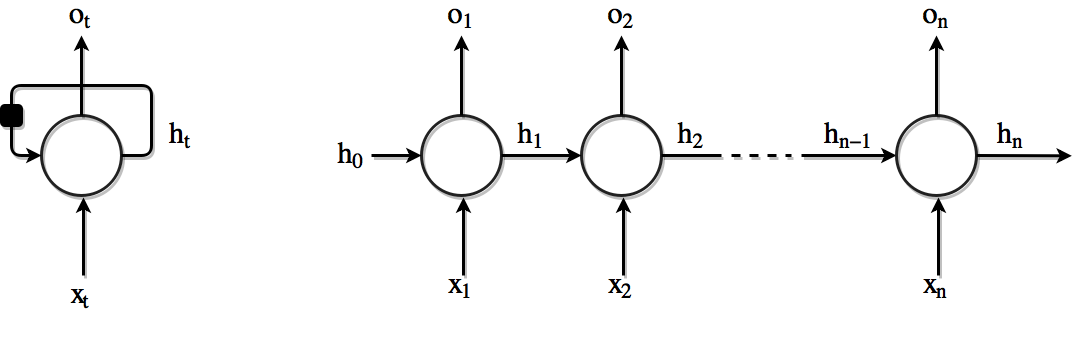
\includegraphics[width=\textwidth]{rnn_folded}
%	\caption[Mạng nơ-ron hồi quy dạng vòng lặp]{Mạng nơ-ron hồi quy dạng vòng lặp}
%	\label{fig_rnn_folded}
%\end{figure}

%Ở dạng dàn trải, một RNN nhận đầu vào là một chuỗi các vector $x_1, x_2,.., x_n$. Tại thời điểm $t (1 \le t \le n)$ vector $x_t$ thuộc chuỗi đầu vào sẽ được đưa vào mạng nơ-ron hồi quy. RNN xử lý vector đó và cập nhật trạng thái ẩn nội tại của nó được đại diện bởi vector $h_t$. Có thể hình dung $h_t$ như là một bộ nhớ lưu giữ thông tin về các vector mà nó đã xử lý cho đến thời điểm $t$. Ở dạng cơ bản nhất, công thức cập nhật trạng thái ẩn của RNN có dạng:



